\section{Singular spectrum and per-lookup cost}
\label{sec:xs_pareto}

\subsection{Singular spectrum}
\label{sec:spectrum}

Figure~\ref{fig:svd_spectrum} shows the normalised singular
values $\sigma_k / \sigma_1$ for eight representative reaction
channels across the nine-nuclide PWR working set plus
$^{235}$U fission. The decay is sharp:
$\sigma_2/\sigma_1 \leq 10^{-1}$ for every channel shown and
$\sigma_6/\sigma_1 < 10^{-14}$ for $^{235}$U fission and
$^{1}$H elastic, reaching double-precision round-off at
rank six.

\begin{figure}[htb]
\centering
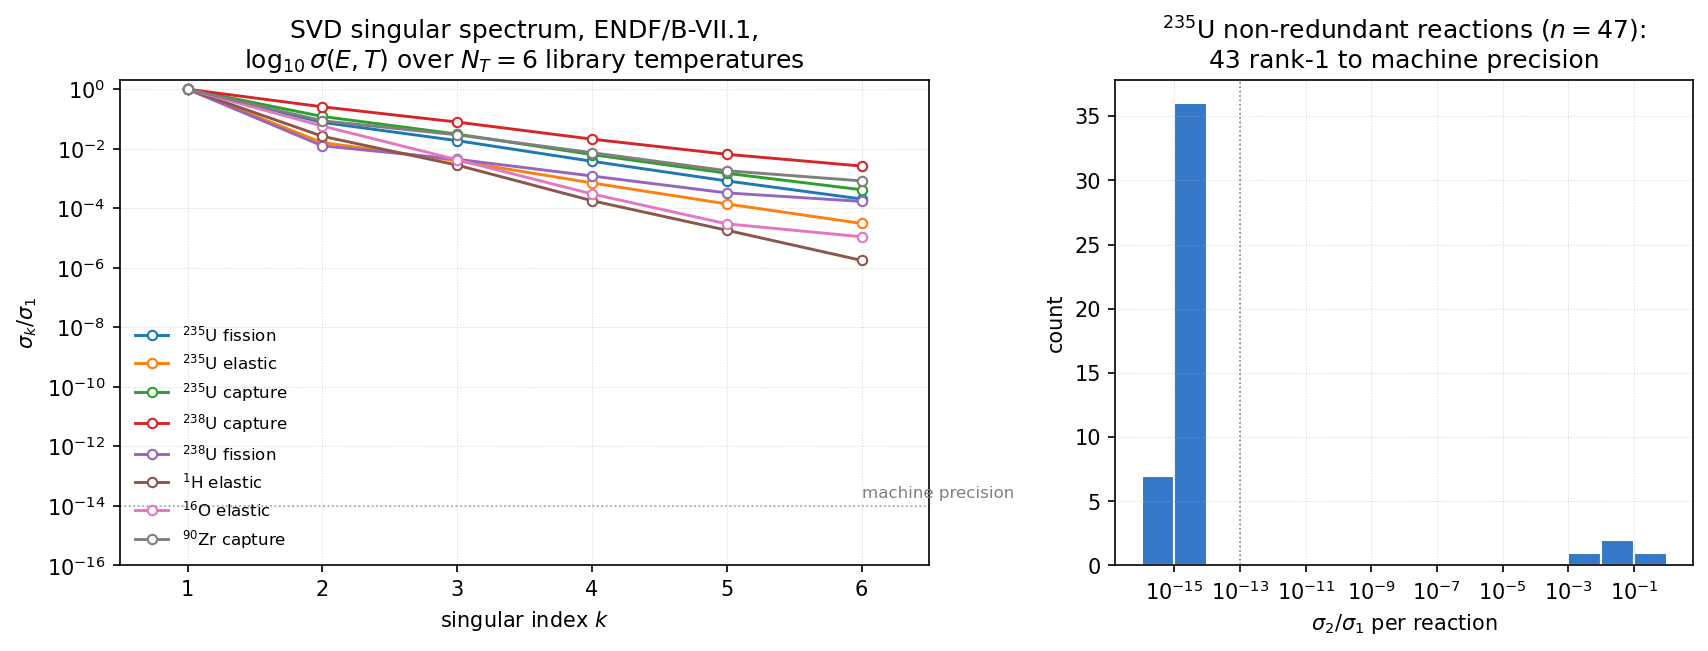
\includegraphics[width=0.99\textwidth]{../outputs/pareto/svd_spectrum.png}
\caption{SVD singular spectrum of $\log_{10}\sigma(E,T)$ for
ENDF/B-VII.1, $N_T = 6$ library temperatures. \emph{Left:}
normalised singular values $\sigma_k/\sigma_1$ for eight
representative channels. The dotted line at $10^{-14}$ marks
double-precision machine epsilon. \emph{Right:} histogram of
$\sigma_2/\sigma_1$ across $^{235}$U's $47$ non-redundant
reaction channels; $43$ are rank-one to machine precision
($\sigma_2/\sigma_1 < 10^{-13}$).}
\label{fig:svd_spectrum}
\end{figure}

$43$ of $47$ non-redundant $^{235}$U reaction channels are
rank-one to machine precision. The four exceptions
(elastic, fission, $(n,2n)$, capture) are the channels with
real structure in both the energy and temperature axes;
those require $k \geq 3$ to reach $\sim\!10^{-3}$ log-RMSE.

\subsection{Per-lookup cost}

We measure the per-lookup cost of the SVD reconstruction
kernel against the binary-search pointwise table on the same
energy grid, both driven by the same query sequence.
Table~\ref{tab:xs_pareto} reports the geometric mean over
eight reactions (MT$=\{2, 18, 102\}$ across
$^{235,238,234}$U) of per-lookup wall time and
log$_{10}$ RMSE against the HDF5 reference.

\begin{table}[htb]
\centering
\caption{XS reconstruction cost and RMSE, geometric mean over
eight reactions. Full energy grid, $T = 294$~K. Desktop
Ryzen~$9800$X3D single-core.}
\label{tab:xs_pareto}
\begin{tabular}{@{}cccc@{}}
\toprule
Rank & ns/lookup & RMSE ($\log_{10}\sigma$) & max $|$err$|$ \\
\midrule
$2$             & $35.9$ & $3.00\times 10^{-2}$ & $9.84\times 10^{-2}$ \\
$3$             & $41.2$ & $7.06\times 10^{-3}$ & $2.86\times 10^{-2}$ \\
$4$             & $43.3$ & $1.83\times 10^{-3}$ & $7.91\times 10^{-3}$ \\
$5$             & $43.4$ & $6.07\times 10^{-4}$ & $3.46\times 10^{-3}$ \\
$6$             & $44.3$ & $1.76\times 10^{-15}$ & $5.58\times 10^{-15}$ \\
Pointwise table & $90.6$ & $0$ (ref) & $0$ (ref) \\
\bottomrule
\end{tabular}
\end{table}

Rank-$6$ reaches machine precision in $44$~ns, $2.0\times$
the pointwise-table per-lookup. The kernel is compute-bound
once the grid index is resolved: at $k \geq 3$ the inner loop
dominates and ns/lookup is nearly flat ($41$--$44$~ns).
Rank-$2$ at $36$~ns is $2.5\times$ the table for a log-decade
RMSE of $3\%$; not adequate inside the RRR
(Sec.~\ref{sec:pwr}). Figure~\ref{fig:per_lookup_cost}
shows the same Pareto visually with the RMSE labels.

\begin{figure}[htb]
\centering
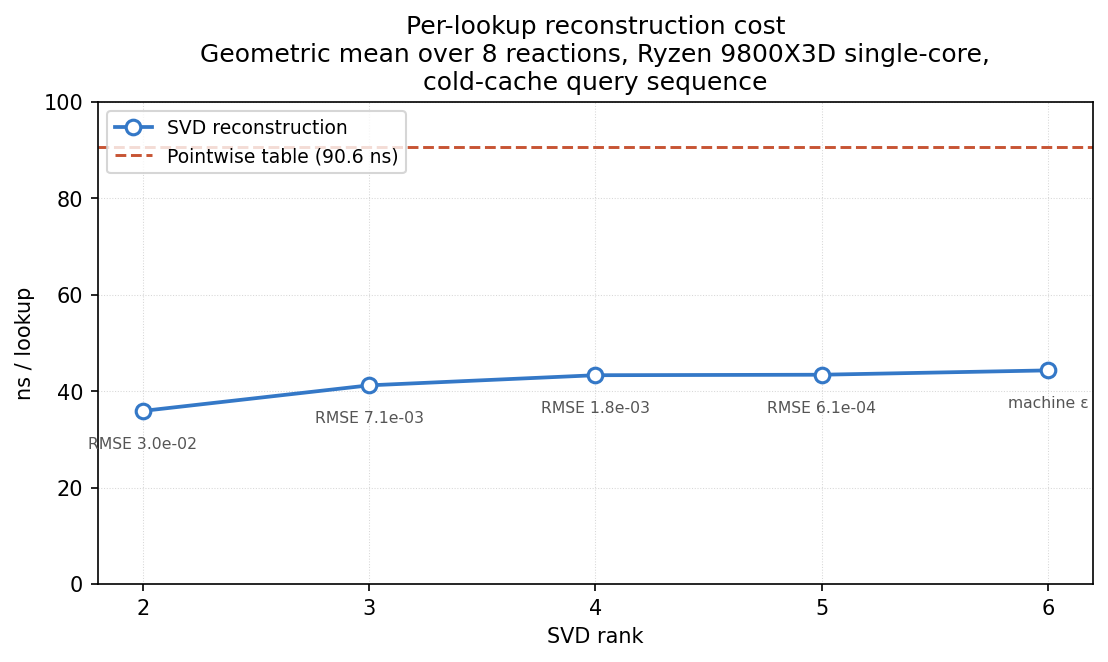
\includegraphics[width=0.76\textwidth]{../outputs/pareto/per_lookup_cost.png}
\caption{Per-lookup reconstruction cost, SVD ranks $2$--$6$
against binary-search pointwise table. Each SVD point
labelled with its $\log_{10}\sigma$ RMSE against the HDF5
reference (machine~$\varepsilon$ at rank $6$).}
\label{fig:per_lookup_cost}
\end{figure}

\paragraph{What this does \emph{not} yet mean.}
This is a kernel benchmark. Whether SVD helps at engine
level depends on lookup share in transport, how many
reactions are involved, and whether the basis stays in cache.
Those are measured in Sections~\ref{sec:pwr} and~\ref{sec:gpu}.

%% ============================================================
